\section{Studio attraverso il reticolo}
Quando della luce incide perpendicolarmente su un reticolo di diffrazione, si viene a creare una figura di interferenza simmetrica rispetto alla direzione di incidenza. La posizione dei punti di interferenza costruttiva (detti massimi) segue la legge \ref{rifrazione}. La luce però non era perfettamente incidente, è dunque possibile considerare l'angolo $\alpha$ di incidenza e scrivere
$$
\sin(\vartheta -\alpha)=n\dfrac{\lambda}{d}
$$
Misurando gli angoli che compaiono in questa relazione, è possibile stimare il passo del reticolo oppure il suo reciproco, di cui in questo caso si conosce il valore con precisione assoluta.
\subsection{Raccolta e analisi dati}
Per svolgere l'esperienza sono stati utilizzati reticoli diversa densità di fenditure, precisamente $300$, $600$ e $1200$ fenditure per millimetro (questi valori corrispondono all'inverso del passo del reticolo).

Per ognuno di essi è stato necessario calibare lo spettrometro in modo che gli angoli dei massimi dello stesso ordine fossero alla stessa distanza angolare dal riferimento $\vartheta_0=\ang{63}\,35'$ nel limite di incertezze sperimentali. La seguente tabella riassume le misure di calibrazione
\begin{table}[h!]
    \centering
    \begin{tabular}{cc}
    \toprule
         Reticolo & $\vartheta_{max}$ (dx/sx)$-\vartheta_0$ \\
         \midrule
         300 & \ang{32}\,30'\\
             & -\ang{32}\,30'\\
        \midrule
         600 &  \ang{46}\,0'\\
          &-\ang{45}\,17'\\
        \midrule
        1200 & \ang{45}\,10'\\
        & -\ang{45}\,2'\\
    \bottomrule
    \end{tabular}
    \caption{}
    \label{tab:my_label}
\end{table}
Dopo questa operazione abbiao misurato gli angoli dei massimi di interferenza meglio individuabili. La seguente tabella mostra i dati raccolti in questa fase
\begin{table}[h!]
    \centering
    \begin{tabular}{cccc}
    \toprule
    Reticolo & $\ang{1}$ ordine & $\ang{2}$ ordine & $\ang{3}$ ordine \\
    \midrule
    300     & \ang{73}\,48’ & \ang{84}\,38'&\ang{96}\,5'\\
    \midrule
    600     &\ang{84}\,32' & \ang{109}\,35' & \\
    \midrule
    1200 & \ang{108}\,35' & &\\
    \bottomrule
    \end{tabular}
    \caption{}
    \label{tab:my_label}
\end{table}
\subsection{Correzione sull'angolo}
La non perpendicolarità della luce incidente può essere corretta introducento l'angolo $\alpha$ il cui valore viene ricavato da considerazioni ottico geometriche da cui si giunge alla seguente relazione
\begin{equation}
    \tan\alpha=\dfrac{\sin\theta_{+}+\sin\theta_{-}}{2-\cos\theta_{+}-\cos\theta_{-}}
\end{equation}
dove $\theta_\pm$ sono gli angoli, a destra e a sinistra, a cui si trovano i massimi della figura di interferenza. Da questa relazione può essere ricavata l'incertezza relativa a questa grandezza che si trova essere
\begin{equation}
\sigma_{\alpha}^{2}=\frac{\left(2 \cos \theta_{+}-\cos \left(\theta_{+}-\theta_{-}\right)-1\right)^{2}+\left(2 \cos \theta_{-}-\cos \left(\theta_{+}-\theta_{-}\right)-1\right)^{2}}{\left(1+\tan ^{2} \alpha\right)^{2}\left(2-\cos \theta_{+}-\cos \theta_{-}\right)^{4}} \sigma_{\theta}^{2}
\end{equation}
La seguente tabella riassume i risultati raccolti
\begin{table}[h!]
    \centering
    \begin{tabular}{ccc}
    \toprule
    Reticolo & $\alpha$ & $\sigma_\alpha$\\
    \midrule
    300     &0' &5' \\
    \midrule
    600     &50' &2'\\
    \midrule
    1200 & 7' & 2' \\
    \bottomrule
    
    \end{tabular}
    \caption{}
    \label{tab:my_label}
\end{table}
\subsection{Verifica della legge di diffrazione \label{paragrafo 3}}
\begin{figure}[h!]
    \centering
    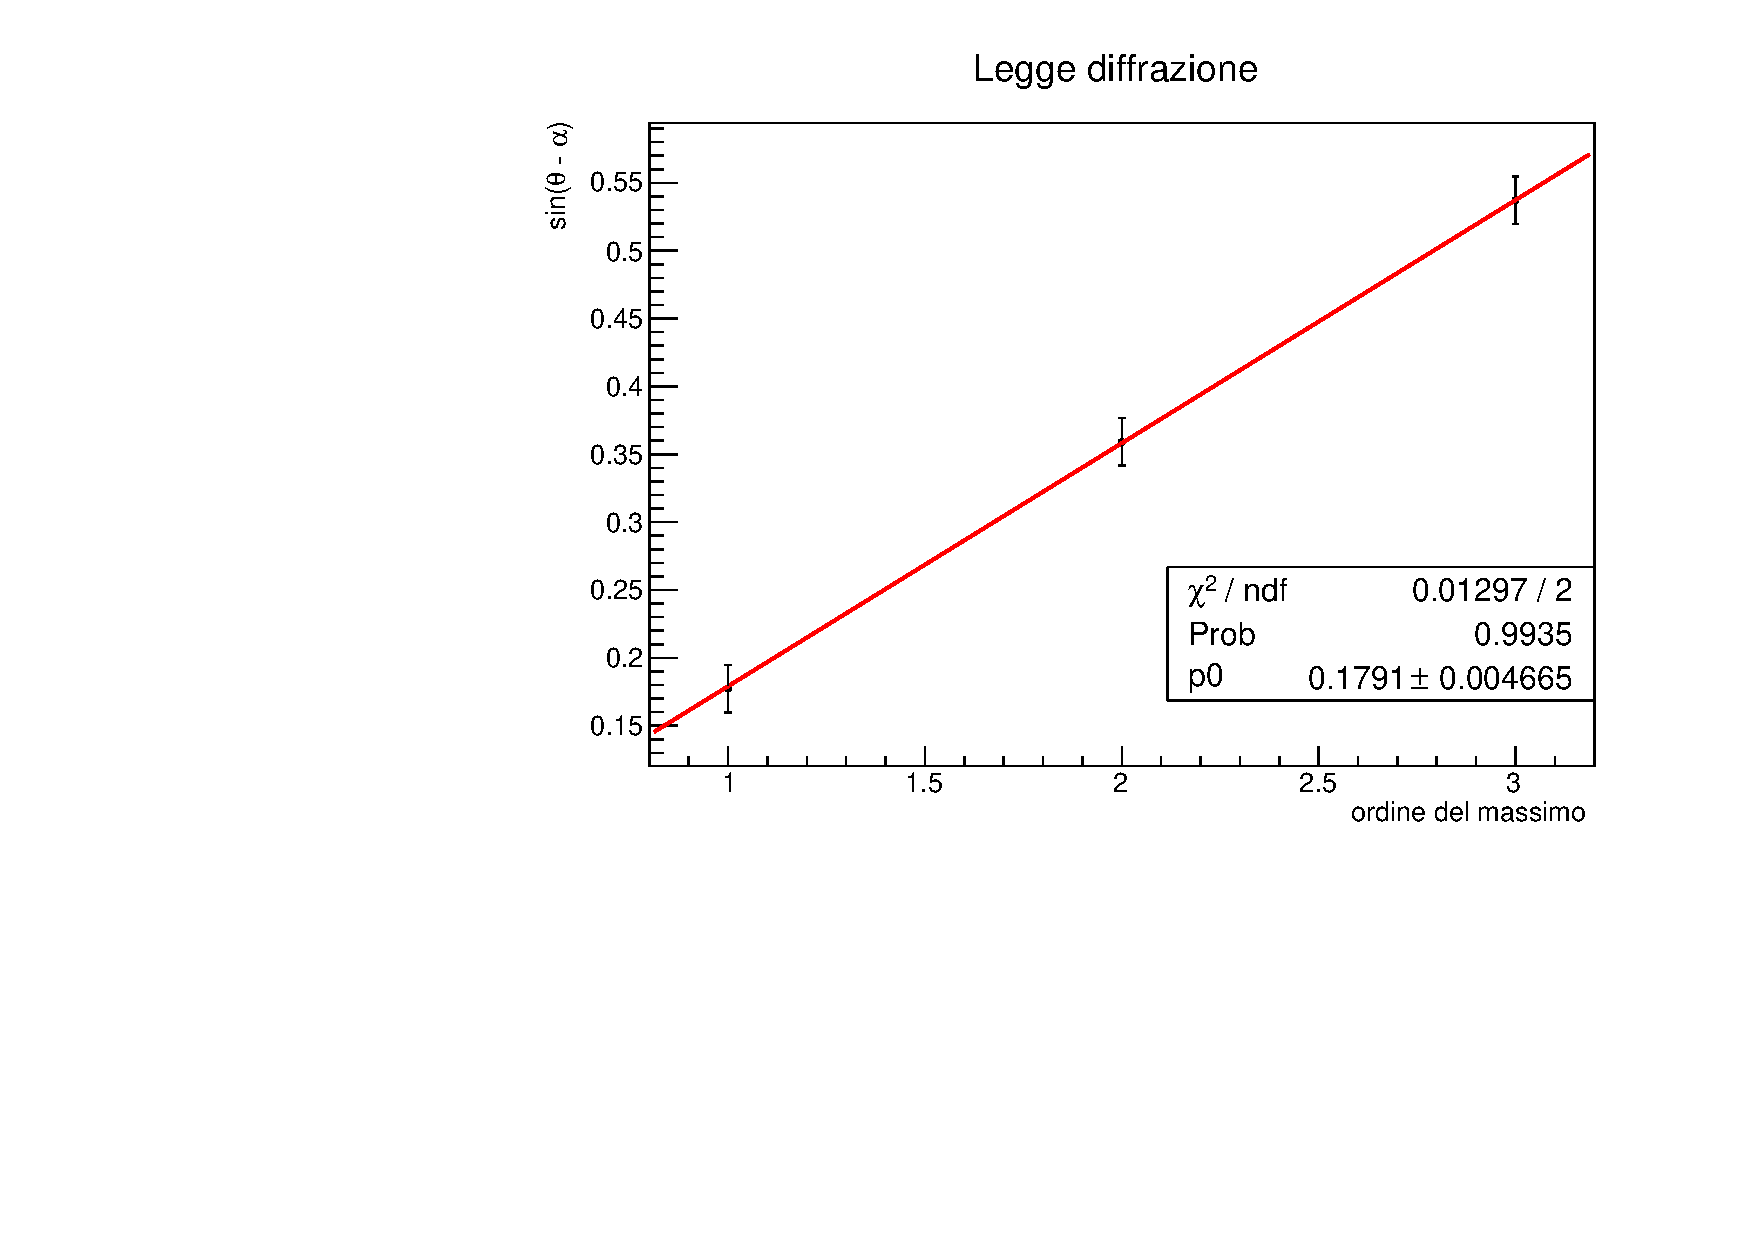
\includegraphics[scale=.6]{Immagini/legge diffrazione.pdf}
    \caption{}
    \label{fit rifrazione}
\end{figure}

Siccome utilizzando il reticolo da $300\,\frac{\text{fend.}}{\text{mm}}$ è possibile ricavare massimi di tre ordini differenti, la stima del suo passo può essere effettuata interpolando l'equazione
$$
\sin(\vartheta-\alpha)=n\dfrac{\lambda}{d}
$$
In questo modo si verifica anche la legge stessa. Chiamato $\beta=\vartheta-\alpha$ l'angolo effettivo del massimo rispetto alla normale del reticolo, si può dire che 
$$
\sigma^2_\beta = \sigma_\alpha^2+\sigma_\vartheta^2
$$
per poi effettuare il fit riportato nella Fig. \ref{fit rifrazione}. Da tale interpolazione si stima il valore caratteristico del reticolo dividendo per $\lambda$
$$
\dfrac{1}{d}=303,8\pm 0,5 \frac{\text{fend.}}{\text{mm}}
$$
Il valore ricavato di $1/d$ non è compatibile con il valore atteso di $300\,\frac{\text{fend.}}{\text{mm}}$ in quanto eseguendo il $t-$test di Student si trova che 
$$
t_s=\dfrac{\hat{\vartheta}-\vartheta_t}{\sigma_\vartheta}=7,6
$$

Questo fa presumere che la legge di diffrazione sia esatta (i dati sperimentali seguono effettivamente una proporzionalità lineare), ma che ci sia un errore nella stima del valore cercato. L’ipotesi più attendibile riguarda un errore nella stima di $\alpha$: dato che una sua variazione di pochi primi comporta un’importante variazione dei risultati, e dato che il supporto del reticolo non era vincolato in modo rigido ma libero di muoversi, si può supporre che nell’atto di misurazione degli angoli tale reticolo si sia leggermente spostato.
\subsubsection{Altri reticoli}
Siccome per gli altri reticoli non disponevamo di sufficienti misure per effettuare un'interpolazione affidabile abbiamo proceduto sitmando i parametri in maniera diretta
$$
\frac{1}{d}=\frac{1}{n \lambda} \sin (\theta-\alpha)
$$
$$
\sigma_{\frac{1}{d}}=\frac{1}{n \lambda} \cos (\theta-\alpha) \sqrt{\sigma_{\theta}^{2}+\sigma_{\alpha}^{2}}
$$
I risultati sono raccolti nella seguente tabella
\begin{table}[h!]
    \centering
    \begin{tabular}{ccc}
    \toprule
    Reticolo $(\frac{\text{fend.}}{\text{mm}})$ & $1/d$ $(\frac{\text{fend.}}{\text{mm}})$ & $\sigma_{\frac{1}{d}}$ $(\frac{\text{fend.}}{\text{mm}})$\\
    \midrule
         600 & 599,2 & 0,4 \\
         1200 &  1200,3 & 0,8\\
    \bottomrule
    \end{tabular}
    \caption{}
    \label{tab:my_label}
\end{table}
\\

In questo caso i valori sono accettabilmente compatibili con quelli attesi e ci permette di confermare la validità della legge di diffrazione, a discapito dell’errata stima fatta in precedenza.